%- Quintile sorted predicted returns (simonian 2019)
%-OLS
% - summaries for coef attribution
%-RF
% - Summary for feat imp
% compare coefficients between feat imp and ols coef
% Sector rotation strat

% \subsection{Hypothesis}
% The overarching objective of this study is captured by Research Questions (a) and (b). For Research Question (a), the hypotheses that follow are literature based ex-ante expectations about (i)the incremental contribution of liquidity and sentiment enhancements, (ii) the comparative predictive performance of RF alternatives and (iii) the practicality of applying these specifications to Sector Rotation Strategy.

% To address Research Question (a), we first benchmark the traditional Fama-French models. Within the training window we anticipate that all factors in the ($C4F$) and ($FF5$) models will remain statistically significant at the 5\% level. These models should yield low in-sample $R^{2}$, due to its linear nature and non-flexibility to adapt to market changes. This expectation reflects the well-documented risk-pricing roles of market excess return, size, value and momentum premiums, together with profitability and investment effects in the $FF5$ \cite{ff5_2015,cahart_1997}. It is also expected that static OLS specifications will underperform out of sample because their constant beta structure cannot readily accommodate regime shifts in liquidity conditions, investor sentiment or other macroeconomic factors.  When the established linear Fama-French models are enhanced by appending liquidity and sentiment proxies, multicollinearity and over parameterisation are likely to inflate standard errors and obscure economic interpretation. Accordingly, it is predicted that most liquidity and sentiment coefficients will be statistically insignificant, leaving the original $C4F$ and $FF5$ factors
% as the only robust drivers. We should also see a reduction both in-sample and out-of-sample fit relative to the linear baselines. The detailed coefficient estimates, significance levels, and economic interpretations for these linear models are intentionally unreported, as doing so would exceed the scope of this study's research questions and would entail presenting an unwieldy number of results across eleven sectors and four model specifications. The full result, however, are available in full in the accompanying GitHub repository.

% Random Forest regressions directly target the nonlinearities that handicap OLS, and therefore is the direct comparison for Research Question (a). By aggregating decision trees, RF models can capture higher-order interactions without specifying it in the variables'functional form, while the boostrapping process and random feature subsampling mitigate overfitting provided hyperparameters are tuned via cross-validation. We therefore hypothesise that RF variants of $C4F$ and $FF5$ will deliver higher in-sample $R^{2}$ and lower out-of-sample mean-squared error than their OLS counterparts. Gains should be largest in volatile or growth-oriented sectors where returns are conditional on threshold effects and regime shifts. Notable sectors to look out for include Information Technology, Communication Services, Financials and Real Estate, based on these sectors' descriptive statisitics indicating volatility. Unlike OLS, RF should benefit from the inclusion of a rich set of liquidity and sentiment variables because correlated predictors are essentially decorrelated across trees. Feature-importance measures are expected to highlight the same first-order drivers identified by linear $t$-statistics, but will additionally reveal interaction effects that linear models cannot represent. However, it is important to note that feature importance scores are not directly comparable with $t$ statistics, thus the statistical significance of feature importance scores cannot be directly inferred. 

% To statisically compare the forecasting performance between all specifications and variations, we have the following hypotheses for the DM test:
% \begin{align}
% d_t &= L\bigl(e^{(1)}_t\bigr) \;-\; L\bigl(e^{(2)}_t\bigr), \\[6pt]
% H_0: &\quad \mathbb{E}\bigl[d_t\bigr] = 0, \\[4pt]
% H_A: &\quad \mathbb{E}\bigl[d_t\bigr] \neq 0.
% \end{align}

% The null hypothesis indicates that the two forecasting methods have equal expected loss (no difference in predictive accuracy) while the alternative hypothesis states that there is a difference in predictive accuracy. In this specific dataset, it is expected that all RF specifications will outperform their OLS counterparts on a statistically significant level. We expect the same to happen with base vs enhanced of the RF models, albeit at smaller magnitudes. Between the C4F and FF5 variations however, it is not expected to yield a statisically significant difference on all sectors. Of course, in the notable sectors listed above, it is also very likely that in those sectors we could reject the null hypothesis, thereby revealing certain characteristics of these sectors for investors.

% For Research Question (b), I hypothesise that ARL applied to the RF based factor forecasts will distill sets of transparent “if-then" rules that will allow for dynamic sector allocations to generate positive active returns relative to the S\&P 500. In particular, we expect that the liquidity and sentiment-enhanced RF-C4F variant will produce the highest cumulative return, alpha, Information Ratio, and Portfolio Sharpe Ratio (at a zero-Sharpe benchmark). This expectation is grounded in recent literature that highlights the pivotal role of momentum, empirical evidence demonstrating that momentum enhances nonparametric forecasting strategies, and studies showing that the FF5 framework is not robust in explaining equity returns \cite{simonian_2019,gu_2020,sarwarff5}. However, it is very likely that for both C4F and FF5, the enhanced variants will outperform their base counterparts in the Sector Rotation strategy.  Enhanced RF-FF5 model will deliver superior risk-adjusted performance to its base counterpart, reflecting the additional information encoded in profitability and investment interactions, while the base RF-C4F model may underperform without these enhancements. Finally, we posit that a constrained implementation—which limits sector deviations from market weights—will preserve the rank order of model performance seen in the unconstrained strategy but offer lower volatility and drawdown, thereby improving the trade-off between active return and active risk.


% %For interpretability, comapre the findings of the pseudo beta to the findings of the current literature

\subsection{Model Interpretability}

After our RF training pipeline, the FI and pseudo-beta are collected. FI shows the contribution of each variable in the RF to excess returns and shown in \cref{tab:feature_importance_rf-baseline-c4f-arl,tab:feature_importance_rf-baseline-ff5-arl,tab:feature_importance_enhanced-rf-c4f-arl_1,tab:feature_importance_enhanced-rf-c4f-arl_2,tab:feature_importance_enhanced-rf-ff5-arl_1,tab:feature_importance_enhanced-rf-ff5-arl_2} in the Appendix. Across the eleven GICS sectors, the RF baseline models display a strikingly uniform importance distribution. In both the C4F and FF5 variants, the excess-market return consistently absorbs the largest share of node split criterion weight (roughly 27-29\%). Size ($SMB$) and value ($HML$) follows, while momentum ($UMD$) and, in the five-factor specification, profitability ($RMW$) and investment ($CMA$) divide the residual importance fairly evenly. The principal difference between C4F and FF5 is minimal: the additional $RMW$ and $CMA$ factors only take a few percentage points from $MKT$, but no variable emerges as a clear new dominant driver. In short, factor contributions are not sector-specific in this analysis, nor does either factor set decisively outshine the other.

%RF base vs RF enhanced
Once the models are enhanced with non-traditional predictors, a surprising shift occurs. The sentiment index of \citeA{wurgler_2007} claims close to 10 \% of total importance, displacing $MKT$ as the single most influential determinant of the forest's splits. By contrast, the two liquidity proxies (share turnover and the Amihud illiquidity ratio) exhibit negligible importance, suggesting that their information is either redundant with the traditional factors or consumed by the sentiment measure. Importantly, the inclusion of sentiment alters the importance without changing the uniformity of all the remaining factors. The traditional excess returns still share the bulk of explanatory power, but sentiment supplies a source of predictability that the baseline models does not have access to. These findings imply that investor psychology is economically meaningful in sector-level return forecasting, whereas common liquidity metrics, though still share uniform weight in importance, adds less value in non-parametric models.

\citeA{simonian_2019} originally proposed the concept of a "pseudo-beta" as a bridge between the predictive strengths of RF and the familiar beta coefficients derived from OLS, arguing that weighting RF variable importances by feature elasticity could yield interpretable analogues of linear factor loadings. From 1998 to 2017, RF models were trained and their RFI were converted into pseudo-beta measures. The pseudo betas for all model specifications are reported in Tables \ref{tab:rfi_statistics_1} to \ref{tab:rfi_statistics_2} in the Appendix. Although these pseudo-beta coefficients do not carry the same statistical guarantees as OLS regression coefficients, they allow finance practitioners that familiar with OLS betas or PCA loadings to interpret black-box ML results in familiar terms. In this framework, a one-unit increase in feature $X$ is associated with a $\beta$-unit change in the target variable $Y$, exactly as in a linear model. Since all of the Fama French factors are represented as percent, an unit change in the feature is a 1\% change. Because these pseudo-beta values are expressed in percentage terms, one must account for the fact that inputs such as excess market returns typically vary by less than 0.1 when interpreting their magnitude.


%Rf base
The RF baseline models confirm that the traditional Fama French factors remain the primary drivers of excess returns across sectors. In both the C4F and FF5 specifications, the RFI profile closely tracks the established ordering of factor contribution in the literature. Market beta still dominates, but the size ($SMB$) and value ($HML$) factors make the largest incremental contributions. The pseudo-beta coefficients suggest that a one percent increase in either factor translates into roughly $0.5$ to $1.0$ percent of additional daily excess return in most sectors, rising to $1.5$ percent in the Consumer Discretionary segment. Momentum ($MOM$) shows a more modest yet systematic effect. When profitability ($RMW$) and investment ($CMA$) are added in $FF5$, their elasticities nearly match that of $MOM$, effectively redistributing importance away from $SMB$ and $HML$ without changing significantly going from sector to sector.

%Rf enhanced
Augmenting the models with liquidity-risk and sentiment variables creates interesting insights. Among the liquidity proxies, turnover ($TURN$), market equity ($ME$), dollar volume ($DVOL$), bid-ask spread ($BASPREAD$), zero-trading days ($ZERODAYS$) and Amihud illiquidity ($ILLQ$), all but $ILLQ$ contribute negligibly: their RFI weights are close to zero, and $ZERODAYS$ is often inactive in sectors such as Materials, Consumer Discretionary, Consumer Staples, Utilities and Real Estate where trading is continuous. By contrast, a one unit increase in $ILLQ$ lifts predicted excess returns by up to $5$ percent in Information Technology and by smaller yet economically meaningful amounts in Health Care, highlighting the reward for bearing illiquidity risk in these sectors. For sentiment factors, the News Sentiment Index consistently shows a stable positive effects, especially in Materials, Industrials, Consumer Discretionary, Financials, Information Technology and Communication Services. This suggests that favourable information about these sectors and individual companies boosts sector-level excess returns. However, it is important to note that the effect is not every economically significant. News Sentiment Scores never go past the range $[-0.5, 0.5]$ and usually increases in 0.05 increments in less volatile periods. Therefore, it is impossible to see a one unit increase in news sentiment, in which we only see a 0.001 percent increase in excess returns. Short-term market fear indices ($VIX_{\text{close}}$) also exert only marginal influence. However, unique in our set of factors is the  enhanced Baker-Wurgler index consistently subtracts from expected returns, indicating that heightened optimism can potentially depress future performance. The characteristic behavior of the enhanced Baker Wurgler index has been documented in prior studies, which reinforces that the pseudo beta accurately conveys the expected directional signal to investors \cite{ung_2023,wurgler_2007}.


\subsection{Model Performance and pseudo beta}
Tables \ref{tab:baseline_ols_c4f} and \ref{tab:baseline_ols_ff5} (in the Appendix) reports the forecasting performance for the eight model specifications for each of the 11 sectors. The base OLS specifications provide only minimal explanatory power for daily sector-level excess returns. In both the C4F and FF5 variants, the baseline models yield an in-sample $R^{2}$ below 1\%, confirming that a purely linear model cannot train on the nonlinear dynamics of almost two decades of the growing equity markets.  Although the MSE and mean-absolute-error (MAE) values reported are numerically small, this is largely due to the low values of daily excess returns (typically the mean is $<0.001\%$).  Notably, for both the C4F and FF5 variants, the Financial sector (40) and especially Real Estate (60) has a high hold-out MSEs (0.003 and 0.01 respectively).  Augmenting the regressions with liquidity risks and sentiment factors improves fit only marginally and Financial/Real Estate errors, while reduced, are still large. Overall, the enhanced OLS models remain vulnerable to market shifts and yield volatile out-of-sample errors, and the results show the limitations of linear factor models for forecasting.

By contrast, the RF frameworks deliver an immediate uplift in predictive accuracy. Even without the enhanced factors, the base RF models (\cref{tab:rf_baseline_c4f,tab:rf_baseline_ff5}) achieve over six times the $R^{2}$ of the OLS specification and reduce the out-of-sample RMSE by approximately two orders of magnitude. The gains are most striking for Real Estate, where RF achieves the second-lowest sectoral hold-out performance despite that sector's return volatility and liquidity.  When liquidity and sentiment are incorporated (\cref{tab:enhanced_rf_c4f,tab:enhanced_rf_ff5}) the fit improves further, yet the incremental error reduction over the baseline RF is modest. A contradicting pattern emerges across factor sets: the C4F specification excels in highly volatile sectors (notably 40 and 60), whereas FF5 produces more uniform errors across the remaining segments.  Taken together with the interpretability results outlined in the previous section, these results confirm that RF creates a robust and transparent foundation for the thesis's signal-generation and sector-rotation framework.  Furthermore, it could be seen that the models' fit and accuracy increase in out-of-sample performance without overfitting on in-sample fit.

The results of the DM tests are reported in \cref{tab:dm_test_combined}. For both the traditional C4F and FF5 baselines, every comparison between RF and OLS models is statistically significant at the 99\% level, except in the Financials sector, where significance is 95\%. Under Hypothesis \ref{hyp:dm2}, we therefore reject $H_{0}$ of equal forecast accuracy in all eleven sectors ($p<0.01$ in ten cases; $p<0.05$ for Financials) and accept $H_{\alpha}$ that RF reduces MSE relative to OLS.  Accordingly, we reject the null hypothesis of equal forecast accuracy between OLS and RF across all sectors.  A negative DM statistic indicates that the model listed first in each column header achieves lower mean squared error (i.e.\ superior forecasting accuracy) than the model listed second. Therefore, RF outperforms OLS in this context.

When comparing RF specifications, augmenting the C4F baseline with liquidity and sentiment factors yields statistically significant improvements (at the 95\% level or better) for Energy, Materials, Industrials, Utilities, and Real Estate, but produces no detectable change for Consumer Discretionary, Consumer Staples, Healthcare, IT, or Communication Services. Hence, with respect to Hypothesis \ref{hyp:dm3}, we reject $H_{0}$ for the first five sectors and cannot reject it for the remaining six, implying that the extra factors add value only where liquidity risk is pronounced or sentiment is less efficiently captured by momentum. A likely explanation is that the Carhart momentum factor already coincide with much of the information contained in investor sentiment measures for these high activity sectors. Indeed, the FI tables in \cref{tab:feature_importance_rf-baseline-c4f-arl} and \cref{tab:feature_importance_enhanced-rf-c4f-arl_1} show that sentiment variables, particularly $\mathrm{VIX}_{\text{close}}$, rank among the most important predictors. Thus, adding explicit sentiment inputs may simply replicate existing momentum patterns, making any forecast improvements insignificant. This interpretation is consistent with \citeA{schmeling_2009}, who finds that a Baker Wurgler sentiment index adds little predictability in markets where momentum effects are pronounced. \citeA{brown_2005} also document that many indirect sentiment proxies move in tandem with momentum returns. \citeA{lee_2000} further observe that, in the Technology and Consumer Staples sectors, sentiment effects are largely embedded within the Carhart momentum factor.  Similarly, enhancing the FF5 model with the same factors delivers significant accuracy gains in all sectors except Communication Services and Real Estate. Consequently, for RF-FF5 we reject $H_{0}$ in nine sectors and fail to reject it in two, suggesting that the profitability ($RMW$) and investment ($CMA$) factors already capture some liquidity and sentiment related effects in those segments. However, existing evidence for this phenomenon is less established in the current literature.  It can be concluded that adding sentiment and liquidity to RF-FF5 does yield statiscally significant improvements in accuracy for nine out of eleven sectors. With RF-C4F showing statistically significant improvements in Communication Services and Real Estate, it is possible that the profitability and investment factors ($RMW$ and $CMA$) in FF5 are capturing dynamics that would otherwise be explained by the liquidity and sentiment variables.

\begin{landscape}
\begin{table}[H]
\centering
\caption{Diebold-Mariano Test Results: Comprehensive Comparison Across Experiments}
\label{tab:dm_test_combined}
\begin{tabular}{lccccccc}
\toprule
Sector & \begin{tabular}[c]{@{}c@{}}RF-C4F\\vs RF-C4F-E\end{tabular} & \begin{tabular}[c]{@{}c@{}}RF-FF5\\vs RF-FF5-E\end{tabular} & \begin{tabular}[c]{@{}c@{}}RF-C4F\\vs OLS-C4F\end{tabular} & \begin{tabular}[c]{@{}c@{}}RF-FF5\\vs OLS-FF5\end{tabular} & \begin{tabular}[c]{@{}c@{}}RF-C4F-E\\vs OLS-C4F-E\end{tabular} & \begin{tabular}[c]{@{}c@{}}RF-FF5-E\\vs OLS-FF5-E\end{tabular} \\
\midrule
Energy & -4.162*** & -1.247 & -5.609*** & -6.122*** & -5.819*** & -5.293*** \\
Materials & -7.245*** & -7.974*** & -5.859*** & -5.791*** & -8.091*** & -8.087*** \\
Industrials & -4.024*** & -6.770*** & -4.411*** & -3.859*** & -6.496*** & -7.008*** \\
Consumer Discretionary & -1.117 & -2.359* & -4.432*** & -3.905*** & -3.821*** & -4.689*** \\
Consumer Staples & -0.547 & -7.022*** & -3.843*** & -4.542*** & -3.601*** & -6.994*** \\
Health Care & -0.714 & -4.447*** & -3.900*** & -4.038*** & -4.081*** & -5.808*** \\
Financials & -4.042*** & -3.124** & -2.394* & -2.571* & -4.233*** & -4.132*** \\
Information Technology & -0.593 & -3.237** & -3.365*** & -2.929** & -3.713*** & -4.141*** \\
Communication Services & -1.781 & -4.619*** & -4.953*** & -4.913*** & -5.294*** & -6.429*** \\
Utilities & 4.723*** & -1.836 & -5.077*** & -4.007*** & -3.394*** & -3.744*** \\
Real Estate & -4.839*** & -0.983 & -4.757*** & -4.196*** & -6.800*** & -3.991*** \\
\bottomrule
\end{tabular}
\begin{tablenotes}
\small
\item Significance levels: *** p $\leq$ 0.001, ** p $\leq$ 0.01, * p $\leq$ 0.05
\end{tablenotes}
\end{table}
\end{landscape}

\subsection{Sector Rotation Strategy}

We evaluate the sector rotation strategy over a hold-out sample of 2018. The strategy's performance is benchmarked against the S\&P500 returns index, which is weighted by market capitalization, computed as the product of share price and total shares outstanding. Many empirical studies benchmark their investment or sector rotation strategies against the S\&P500 due to its status as the primary large-cap U.S. equity market proxy, such as \citeA{sawar_2017} where the authors uses S\&P500 as a benchmark for a sector rotation strategy using FF5 alphas. As detailed in \cref{sec:data}, 2018 was characterized by heightened market volatility and adverse macroeconomic shocks. Consequently, the cumulative return of the S\&P500 over this period was $-6.24\%$ \footnote{This paper omits the data point on 30-12-2018 since on 30/12/2018, there are no next day signal to be used for forecasting (next trading day is on 2019). Therefore the reported returns is different, at -7,03\%. If this data point is included, the cumulative return of the S\&P500 over this period was $-6.24\%$ indeed.}. The cumulative return of the equal-weighted portfolio is reported in Table \ref{tab:return_stats_1} and Figure \ref{fig:eq_w_cum_ret_plot}. While the S\&P500 weighs every security based on their market capitalization, the equal-weighted portfolio assigns equal weight to each security, every trading day. It can be seen that a passive buy and hold equal-weighted portfolio, though operated at a loss in 2018, still beat the S\&P500 index by 4.79\%. This will be a common theme throughout this results section. In 2018, due to market conditions, a negative returns does not mean that the strategy is performing poorly. However, if any strategy yields a positive return, it would be considered an outstanding performance by the model underlying that strategy.

\begin{figure}[H]
    \centering
    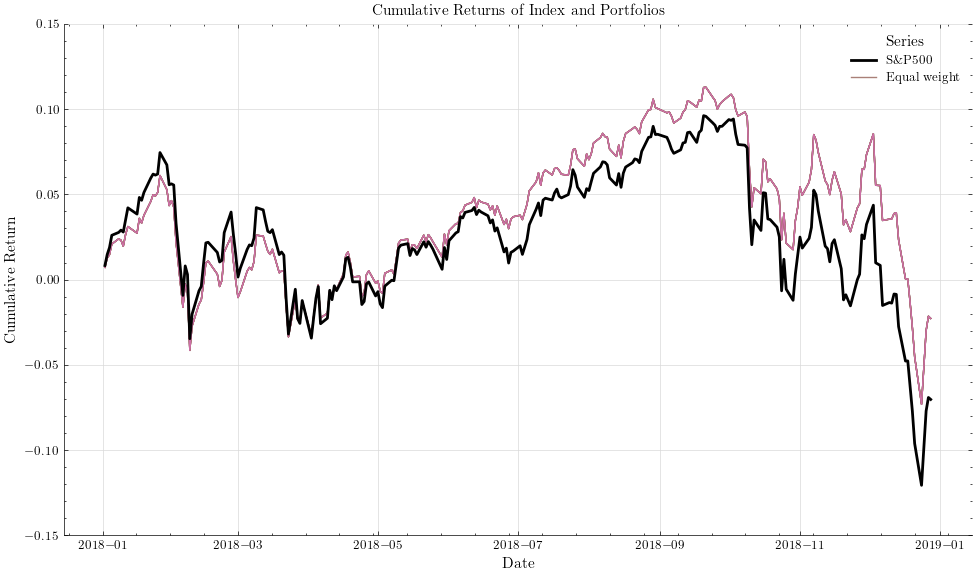
\includegraphics[width=\textwidth]{plots/results/equal_w_cum_ret_plot.png}
    \caption{Cumulative returns of S\&P500 and equal weight sector rotation strategies (2018)}\label{fig:eq_w_cum_ret_plot}
\end{figure}


\begin{table}[ht]
\centering
\caption{Descriptive Statistics of Index and Portfolio Returns}
\label{tab:return_stats_1}
\begin{tabular}{lrrrrrrr}
\toprule
{} & \multicolumn{1}{c}{Cumulative} & \multicolumn{1}{c}{Annualised} & \multicolumn{1}{c}{Annualised} & \multicolumn{1}{c}{Alpha} & \multicolumn{1}{c}{Information} & \multicolumn{1}{c}{PSR} & \multicolumn{1}{c}{PSR} \\
{} & \multicolumn{1}{c}{Return} & \multicolumn{1}{c}{Return} & \multicolumn{1}{c}{Volatility} & {} & \multicolumn{1}{c}{Ratio} & \multicolumn{1}{c}{(S*=0)} & \multicolumn{1}{c}{(S*=0.1)} \\
\midrule
S\&P500 & -7.03\% & -7.08\% & 17.06\% & 0.00\% & -- & -- & -- \\
equal\_weight & -2.27\% & -2.29\% & 15.39\% & 4.79\% & 0.29 & 0.43 & 0.03 \\
\bottomrule
\end{tabular}
\end{table}

The cumulative return chart for the in \cref{fig:cum_ret_plot} together with the summary statistics in \cref{tab:unconstr} shows the effectiveness of the active unconstrained sector rotation strategies relative to a passive S\&P 500 benchmark buy and hold strategy. While the index declined by 7.03\% over 2018\footnote{Due to omitted data on 30/12/2018, 2018 period ends on 29/12/2018.}, 7 out of 8 models specifications outperformed the S\&P500 index, and 4 out of 8 specifications made positive returns despite the market conditions. The plot further shows that these active portfolios not only outperformed during the steady upswing through September but also successfully adjusted to the sudden sell off and increased volatility from mid-October onward, thereby dampening the loss.

A closer inspection reveals three surprises. First, the top three performers are all RF specifications, yet the fourth-best is an OLS specification. RF-C4F-E is the best specification, achieving a cumulative return of 5.19\%, translating into an alpha of 12.31\%, an IR of 0.29 and a PSR of 0.97 at the 0.0 Sharpe benchmark.  Second, among RF variants the RF-FF5 variant outperforms its liquidity and sentiment enhanced variant. Opposite to that, the RF-C4F variant yield negative returns and performed worse than the enhanced OLS-FF5-E variant, while its enhanced RF-C4F-E version is the best performing model. Third,  the only portfolio that underperformed the index was the OLS-FF5 (-10.66\%), while its enhanced specification is the only OLS model that generates a positive return, which confirms that both the additional liquidity and sentiment factors are crucial when momentum is missing. Another interesting observation is the RF enhanced models that are C4F variants yield better than their FF5 counterpart. This is probably due to momentum having a particularly strong effect in the macroeconomic environment of 2018, and profitability and investment factors delivered little incremental information.

The constrained strategy, which its statistics are reported in \cref{tab:constr} and \cref{fig:constr_cum_ret_plot}, shows a much more conservative approach to sector weight attribution. Evidently, \cref{fig:constr_cum_ret_plot} shows a much more tight clustering around the S\&P 500, while the unconstrained strategy fans out more. We could see in \cref{tab:constr} that, as expected, the order of the model performance stays exactly the same as the unconstrained model. An advantage of this strategy is that even for OLS models that underperformed against the S\&P500 in unconstrained strategy, the constrained strategy still outperformed the index. Even OLS-FF5 models, which had an active return of -3.58\%, had a positive return of 1.55\% in the constrained strategy. Similarly, OLS-C4F received a bump in active return of 2.2\%, comparing to the unconstrained strategy. What is surprising is that OLS-C4F-E got lower active returns in the unconstrained strategy (3.2\%), compared to a 4.57\% increase in active returns in the constrained strategy. However, with lower risks comes lower returns. With the top 4 models, the unconstrained strategy got anywhere from 3 to 5\% more active returns than the constrained strategy.

However, implementing these models in actual trading applications requires much more than looking at raw return percentages. Each winning specification shows an IR of only 0.2-0.3, meaning that for every unit of active risk the strategy earns merely 0.2 to 0.3 units of excess return. This level of IR is considered modest at best, since institutional managers typically seek IRs above 0.5 to justify the costs and capacity constraints of active rotation \cite{gratton_2025}. The probabilistic Sharpe ratio at $S^{*} = 0$  with values around 40-60\% implying low confidence that the true Sharpe is larger than zero. In practice, one would prefer PSRs above 90\% at the target Sharpe to ensure robustness against estimation error. It essentially tells investors how likely they will make a positive return relative to the risk taken. In this case, we cannot reject the null hypothesis of Hypothesis \ref{hyp:psr} that the true Sharpe ratio is statistically different than zero at a 90\% confidence level. This is understandable given the volatility profile of 2018, where it is extremely uncertain that there would be any positive returns for any strategy. When we refer to the descriptive statistics of 2018, we could see how risky the market is.  Further research, with more computational resources could extend these strategies on a longer horizon (for example, using hold out set of 2016-2018), to have a more accurate outlook on the performance of these underlying models in less volatile periods.



% - Incredible results. Looking at the fig we could see that almost all of  the active strategies are outperforming the buy and hold index strategy. First four models, in a year where Sp500 index loses 7.03%, our strategy were able to hedge against that and even made positive returns. Only one model out of 8 lost against the index
% - In the fig we see that even  the plunge from mid october and volatile times at the end of the year , our models adjusted to that extremely well and generate signals that could hedge against the liquidity risk and sentiment shift
% - Looking closer: top 3 models are rf specification, but extremely surprising that 4rth is ols. Looking deeper in the top 4, c4f enhanced performed best with the cummulative ret =5.19\%, achieving an active return of 12.31\% . surprising that c4f is on top not ff5 {WHY DO YOU THINK c4f is on top not ff5}. even more surprising is that RF-FF5 seems to beat RF-FF5-E. {WHY IS THIS THE CASE}, with 11.44 active return comapred to 10.65\% active return. Most surpirasing of all, however, is that the 4rth place is not rf but an ols model, specifically OLS-FF5-E {WHY IS THIS POSSIBLE?}

% - Bottom 4 models: RF-C4F lost money {WHY enhanced do so good but base lost?}. Contrary to the hypothesis, OLS base models performed worse than the OLS enhanced, specifically c4f >ff5. OLS-FF5 is the only one that lost money {WHY?}



\begin{figure}[H]
    \centering
    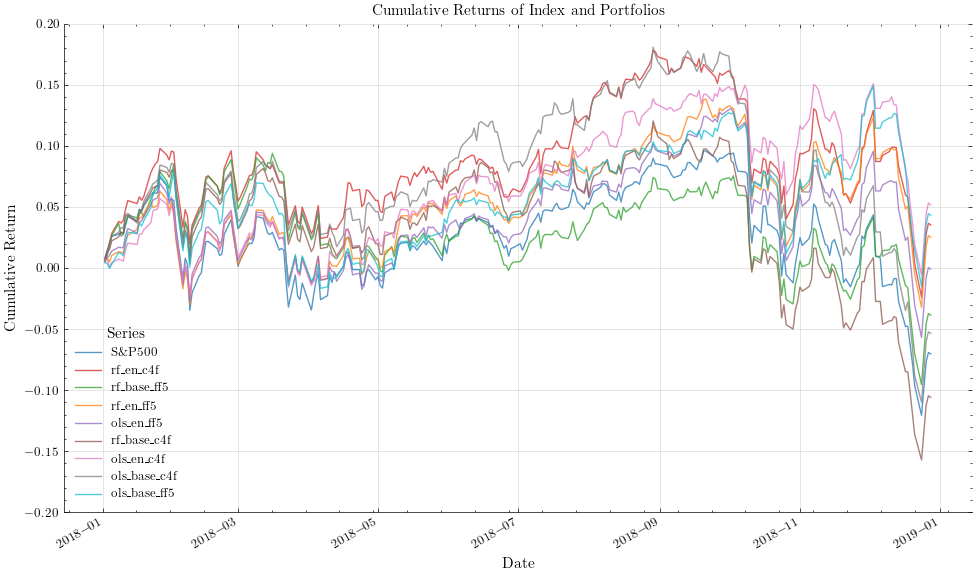
\includegraphics[width=\textwidth]{plots/results/cum_ret_plot.png}
    \caption{Cumulative returns of S\&P500 and Unconstrained sector rotation strategy (2018)}\label{fig:cum_ret_plot}
\end{figure}



% \begin{table}[ht]
% \centering
% \caption{Descriptive Statistics of Index and Portfolio Returns}
% \label{tab:unconstr}
% \begin{tabular}{lrrrrrrr}
% \toprule
% {} & \multicolumn{1}{c}{Cumulative} & \multicolumn{1}{c}{Annualised} & \multicolumn{1}{c}{Annualised} & \multicolumn{1}{c}{Alpha} & \multicolumn{1}{c}{Information} & \multicolumn{1}{c}{PSR} & \multicolumn{1}{c}{PSR} \\
% {} & \multicolumn{1}{c}{Return} & \multicolumn{1}{c}{Return} & \multicolumn{1}{c}{Volatility} & {} & \multicolumn{1}{c}{Ratio} & \multicolumn{1}{c}{(S*=0)} & \multicolumn{1}{c}{(S*=0.1)} \\
% \midrule
% S\&P500 & -7.03\% & -7.08\% & 17.06\% & 0.00\% & -- & -- & -- \\
% rf\_en\_c4f & 5.19\% & 5.23\% & 15.72\% & 12.31\% & 0.29 & 0.97 & 0.61 \\
% rf\_base\_ff5 & 4.33\% & 4.36\% & 16.45\% & 11.44\% & 0.28 & 0.95 & 0.57 \\
% rf\_en\_ff5 & 3.54\% & 3.57\% & 16.55\% & 10.65\% & 0.29 & 0.95 & 0.55 \\
% ols\_en\_ff5 & 2.53\% & 2.55\% & 16.27\% & 9.63\% & 0.28 & 0.95 & 0.53 \\
% rf\_base\_c4f & -0.08\% & -0.08\% & 16.10\% & 7.00\% & 0.26 & 0.93 & 0.48 \\
% ols\_en\_c4f & -3.85\% & -3.89\% & 16.48\% & 3.20\% & 0.22 & 0.89 & 0.38 \\
% ols\_base\_c4f & -5.34\% & -5.38\% & 17.23\% & 1.70\% & 0.21 & 0.86 & 0.33 \\
% ols\_base\_ff5 & -10.58\% & -10.66\% & 17.14\% & -3.58\% & 0.15 & 0.78 & 0.22 \\
% \bottomrule
% \end{tabular}
% \end{table}


% \begin{table}[ht]
% \centering
% \caption{Descriptive Statistics of Index and Portfolio Returns}
% \label{tab:constr}
% \begin{tabular}{lrrrrrrr}
% \toprule
% {} & \multicolumn{1}{c}{Cumulative} & \multicolumn{1}{c}{Annualised} & \multicolumn{1}{c}{Annualised} & \multicolumn{1}{c}{Alpha} & \multicolumn{1}{c}{Information} & \multicolumn{1}{c}{PSR} & \multicolumn{1}{c}{PSR} \\
% {} & \multicolumn{1}{c}{Return} & \multicolumn{1}{c}{Return} & \multicolumn{1}{c}{Volatility} & {} & \multicolumn{1}{c}{Ratio} & \multicolumn{1}{c}{(S*=0)} & \multicolumn{1}{c}{(S*=0.1)} \\
% \midrule
% S\&P500 & -7.03\% & -7.08\% & 17.06\% & 0.00\% & -- & -- & -- \\
% rf\_en\_c4f & -0.05\% & -0.05\% & 15.22\% & 7.03\% & 0.30 & 0.94 & 0.51 \\
% rf\_base\_ff5 & -0.29\% & -0.29\% & 15.39\% & 6.79\% & 0.30 & 0.93 & 0.50 \\
% rf\_en\_ff5 & -0.52\% & -0.53\% & 15.48\% & 6.55\% & 0.31 & 0.93 & 0.49 \\
% ols\_en\_ff5 & -0.83\% & -0.83\% & 15.45\% & 6.25\% & 0.30 & 0.93 & 0.48 \\
% rf\_base\_c4f & -1.59\% & -1.61\% & 15.42\% & 5.47\% & 0.29 & 0.92 & 0.46 \\
% ols\_en\_c4f & -2.71\% & -2.73\% & 15.43\% & 4.35\% & 0.27 & 0.91 & 0.43 \\
% ols\_base\_c4f & -3.16\% & -3.18\% & 15.66\% & 3.90\% & 0.27 & 0.91 & 0.42 \\
% ols\_base\_ff5 & -4.80\% & -4.84\% & 15.65\% & 2.24\% & 0.23 & 0.89 & 0.37 \\
% \bottomrule
% \end{tabular}
% \end{table}

%NEWWWWWWWWWWWWWWWW
\begin{table}[H]
\centering
\caption{Index and Portfolio Returns: Unconstrained Strategy}
\label{tab:unconstr}
\begin{tabular}{lrrrrrrr}
\toprule
{} & \multicolumn{1}{c}{Cumulative} & \multicolumn{1}{c}{Annualised} & \multicolumn{1}{c}{Annualised} & \multicolumn{1}{c}{Alpha} & \multicolumn{1}{c}{Information} & \multicolumn{1}{c}{PSR} & \multicolumn{1}{c}{PSR} \\
{} & \multicolumn{1}{c}{Return} & \multicolumn{1}{c}{Return} & \multicolumn{1}{c}{Volatility} & {} & \multicolumn{1}{c}{Ratio} & \multicolumn{1}{c}{(S*=0)} & \multicolumn{1}{c}{(S*=0.1)} \\
\midrule
S\&P500 & -7.03\% & -7.08\% & 17.06\% & 0.00\% & -- & -- & -- \\
RF-C4F-E & 5.19\% & 5.23\% & 15.72\% & 12.31\% & 0.29 & 0.61 & 0.10 \\
RF-FF5 & 4.33\% & 4.36\% & 16.45\% & 11.44\% & 0.28 & 0.59 & 0.09 \\
RF-FF5-E & 3.54\% & 3.57\% & 16.55\% & 10.65\% & 0.29 & 0.57 & 0.08 \\
OLS-FF5-E & 2.53\% & 2.55\% & 16.27\% & 9.63\% & 0.28 & 0.55 & 0.07 \\
RF-C4F & -0.08\% & -0.08\% & 16.10\% & 7.00\% & 0.26 & 0.49 & 0.05 \\
OLS-C4F-E & -3.85\% & -3.89\% & 16.48\% & 3.20\% & 0.22 & 0.40 & 0.03 \\
OLS-C4F & -5.34\% & -5.38\% & 17.23\% & 1.70\% & 0.21 & 0.37 & 0.03 \\
OLS-FF5 & -10.58\% & -10.66\% & 17.14\% & -3.58\% & 0.15 & 0.25 & 0.01 \\
\bottomrule
\end{tabular}
\end{table}

\begin{figure}[H]
    \centering
    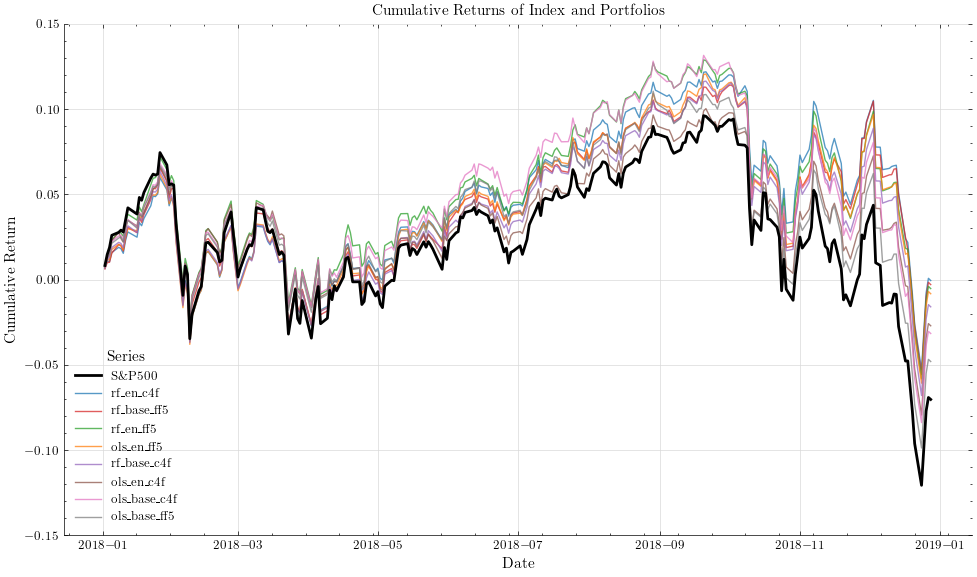
\includegraphics[width=\textwidth]{plots/results/contrained_cum_ret_plot.png}
    \caption{Cumulative returns of S\&P500 and Constrained sector rotation strategies (2018)}\label{fig:constr_cum_ret_plot}
\end{figure}

\begin{table}[H]
\centering
\caption{Index and Portfolio Returns: Constrained Strategy}
\label{tab:constr}
\begin{tabular}{lrrrrrrr}
\toprule
{} & \multicolumn{1}{c}{Cumulative} & \multicolumn{1}{c}{Annualised} & \multicolumn{1}{c}{Annualised} & \multicolumn{1}{c}{Alpha} & \multicolumn{1}{c}{Information} & \multicolumn{1}{c}{PSR} & \multicolumn{1}{c}{PSR} \\
{} & \multicolumn{1}{c}{Return} & \multicolumn{1}{c}{Return} & \multicolumn{1}{c}{Volatility} & {} & \multicolumn{1}{c}{Ratio} & \multicolumn{1}{c}{(S*=0)} & \multicolumn{1}{c}{(S*=0.1)} \\
\midrule
S\&P500 & -7.03\% & -7.08\% & 17.06\% & 0.00\% & -- & -- & -- \\
RF-C4F-E & -0.05\% & -0.05\% & 15.22\% & 7.03\% & 0.30 & 0.48 & 0.05 \\
RF-FF5 & -0.29\% & -0.29\% & 15.39\% & 6.79\% & 0.30 & 0.48 & 0.05 \\
RF-FF5-E & -0.52\% & -0.53\% & 15.48\% & 6.55\% & 0.31 & 0.47 & 0.05 \\
OLS-FF5-E & -0.83\% & -0.83\% & 15.45\% & 6.25\% & 0.30 & 0.46 & 0.05 \\
RF-C4F & -1.59\% & -1.61\% & 15.42\% & 5.47\% & 0.29 & 0.44 & 0.04 \\
OLS-C4F-E & -2.71\% & -2.73\% & 15.43\% & 4.35\% & 0.27 & 0.41 & 0.04 \\
OLS-C4F & -3.16\% & -3.18\% & 15.66\% & 3.90\% & 0.27 & 0.40 & 0.03 \\
OLS-FF5 & -4.80\% & -4.84\% & 15.65\% & 2.24\% & 0.23 & 0.36 & 0.03 \\
\bottomrule
\end{tabular}
\end{table}

